\documentclass{misc/theme}
\usepackage{wallpaper}
\usepackage{tabu,longtable,booktabs,array}
\def\changemargin#1#2{\list{}{\rightmargin#2\leftmargin#1}\item[]}
\let\endchangemargin=\endlist 
\newcommand{\block}[1]{\vspace{1.4cm}\begin{changemargin}{2.5cm}{2.5cm}\large\textit{#1}\end{changemargin}\vspace{0.6cm}}
\newcommand{\fakesection}[1]{%
  \par\refstepcounter{section}% Increase section counter
  \sectionmark{#1}% Add section mark (header)
  \addcontentsline{toc}{section}{\protect\numberline{\thesection}#1}% Add section to ToC
  % Add more content here, if needed.
}
\ThisCenterWallPaper{0.7}{misc/cover.png}
\usepackage{microtype} % Better word wrapping
  \usepackage{color}
\usepackage{xcolor}
\usepackage{hyperref}
\definecolor{blue}{rgb}{0.01, 0.28, 1.0}
\definecolor{lightgray}{rgb}{0.95, 0.95, 0.95}
\hypersetup{colorlinks=true, urlcolor=blue, citecolor=blue, filecolor=blue, linkcolor=blue}
\usepackage{afterpage}
\pagecolor{lightgray}\afterpage{\nopagecolor}
\usepackage[firstpage=true]{background}
\def\Step{0.1cm}
\tikzset{dotted lines/.style={black, loosely dotted,  thick}}
\backgroundsetup{
scale=1,
angle=0,
position={0,0},
contents={
\begin{tikzpicture}[remember picture,overlay]
\draw[dotted lines,step=\Step,help lines]
  (-10,-30) grid  (20,10);
  \end{tikzpicture}
  }
}
\usepackage[font={footnotesize}]{caption}
\usepackage[ruled,vlined]{algorithm2e}
\newenvironment{snippet}[1][htb]
  {\renewcommand{\algorithmcfname}{Code Snippet}% Update algorithm name
   \vspace{0.3cm}\begin{algorithm}[#1]%
  }{\end{algorithm}\vspace{0.3cm}}
\usepackage{array}
\usepackage{tabu}
\usepackage{float}
\usepackage[all]{hypcap}
\usepackage{etoolbox}
\usepackage{xfrac}
\usepackage{fancyvrb}
\makeatletter
\patchcmd{\@BVerbatim}
  {\BVerbatim@font}
  {\BVerbatim@font\footnotesize}
  {}{}
\makeatother

%%% Authors
\addAuthor{Micha\"el}{Dooreman}{}
\addAuthor{Bruno}{Vandekerkhove}{}

%%% Title page
\casename{Advanced Programming Languages for A. I.}
\phasenumber{Micha\"el Dooreman \& Bruno Vandekerkhove}
\phasename{}
\academicyear{2019}
\newcommand{\tbd}{\textbf{To be discussed}}

%%%
%%% Start Document
%%%
\begin{document}
\maketitle
\tableofcontents

%
% Introduction
%

% \fakesection{Introduction}
\block{In the past decades much research has been done on the characterization and resolution of constraint satisfaction - and constraint optimization problems. This report discusses three challenges ; Sudoku puzzles, Hashiwokakero and a scheduling problem.}

%
% Sudoku
% 

\section{Sudoku}

Sudoku is a well-known puzzle game which needs no introduction. It is typically modelled as a constraint satisfaction problem through the use of \texttt{all\_different} constraints on rows, columns and blocks. Such global inequalities tend to improve upon the use of binary inequalities. The constraint generating code\footnote{\texttt{ECLiPSe} and \texttt{CHR} implementations are available in \texttt{/sudoku/model/classic.pl} and in \texttt{/sudoku/chr/model/classic.pl}.} is fairly trivial and needn't be detailed here. \\\par

There are several other ways one could model Sudoku. The widely cited study by Helmut Simonis \cite{article:simonis} and subsequent studies provide some ideas. Four \textit{`dual'} models, two approaches based on a boolean characterisation, a combination of models provided by Laburthe, a model enforcing the singular occurrence of every value in every row, column and block, as well as a model with nothing but channeling constraints were considered\footnote{These are implemented with ECLiPSe in the \texttt{/sudoku/eclipse/model/} directory, and some CHR versions are in \texttt{/sudoku/chr/model/}.}. Tests were run on the provided puzzles\footnote{\texttt{/sudoku/benchmarks/benchmarks.pl} provides automatic benchmarking code.} as well as some minimum puzzles provided by Gordon Royle\footnote{\href{http://rotor.di.unipi.it/cisterni/Shared\%20Documents/minsudoku.html}{These are available online.}}. These are puzzles with a minimal amount of pre-filled cells (17 to be precise \cite{article:mcguire}), which does not mean that they are harder to solve. \\\par

The dual models hold a $N\times N$ array with all the decision variables. Whereas in the classic viewpoint the rows, columns and values of this array correspond to those of the input puzzle, every one of the four dual models changes their roles. The first two switch the role of rows or columns with those of values. In the third model every row and column of the array corresponds to a block and a position. In the fourth dual model every row represents a block, every column a value and every value a position within a block. For each of them it was harder to implement the necessary constraints, usually necessitating the use of auxiliary variables together with appropriate channeling constraints.\\\par  

In one of his works Laburthe discusses various rules that can be used to resolve Sudoku puzzles, after which he details three models that he associates with the rules \cite{article:laburthe}. He ends up proposing a model for every level of difficulty of the input puzzle. An attempt was made at implementing his recommendation for `difficult' puzzles. It decreased the average number of backtracks but increased the runtime. \\\par

The boolean models include the natural combined model \cite{article:natural} and a more intuitive characterisation resembling an integer programming - or a SAT model \cite{article:sat} (using \href{http://eclipseclp.org/doc/bips/lib/ic_global/occurrences-3.html}{\texttt{occurrences/3}} instead of sums, disjunctions and conjunctions). Both of them have $N\times N\times N$ boolean variables $b_{rcv}$ which are true if the cell at row $r$ and column $c$ holds the value $v$. The natural combined model was cumbersome to implement and performed badly. It was introduced together with an algorithm which was tailored after it, and a constraint for unequality of lists isn't really supported by ECLiPSe\footnote{A custom-made implementation as well as the \href{https://eclipseclp.org/doc/bips/kernel/termcomp/TE-2.html}{\texttt{$\sim$=/2}} constraint which checks if two terms can be unified were tried. Channeling back to integers with \href{http://eclipseclp.org/doc/bips/lib/ic_global/bool_channeling-3.html}{\texttt{ic\_global:bool\_channeling/3}} worked better (ironically).}.\par
Note that it is usually not recommended to use a boolean model when integers can be used instead (as pointed out by Rossi \cite{book:rossi}).\\\par
% Rossi is p. 393

The last two models were found to be the most performant. The first makes use of the previously mentioned \href{http://eclipseclp.org/doc/bips/lib/ic_global/occurrences-3.html}{\texttt{occurrences/3}} constraint to make every value occur just once in every row, column and block. 
\par The second one generates nothing but channeling constraints. It has been demonstrated that this can provide good results despite such constraints being less `tight' than \texttt{all\_different} constraints\footnote{\textit{``The reason for this difference is that the primal not-equals constraints detect singleton variables (i.e. those variables with a single value), the channelling constraints detect singleton variables and singleton values (i.e. those values which occur in the domain of a single variable), whilst the primal all-different constraint detects global consistency (which includes singleton variables, singleton values and many other situations)"}\cite{article:channeling}}. When Dot\'u discussed it he was considering QuasiGroups \cite{article:quasi}. This was extended\footnote{The code lies in \texttt{sudoku/model/channeling.pl} in which a flag called \texttt{extended} can be used to opt for one of two variants.} to Sudoku puzzles by making use of three instead of two dual models (since blocks need to be considered as well). The variant in which channeling constraints between all models (one primal, three dual) are generated performed better than the one in which only channeling constraints between the primal and every dual model are applied. These variants are analogous to what Dot\'u referred to as \textit{`trichanneling'} and \textit{`bichanneling'}.

\subsection{Experiments}

Number of backtracks and running time for most of the models are displayed in table \ref{tab:res1}. Removal of \textit{`big'} (\texttt{all\_different}) constraints in the classic model\footnote{In his study Demoen gives several \textit{Missing(6)} examples, models in which 6 of the \texttt{all\_different} constraints are removed. \textit{Missing(7)} models aren't Sudoku, and because of the stark rise in number of backtracks no further experimentation with the removal of `\textit{small}' constraints was done. The \texttt{eliminate\_redundancy} flag can be used to toggle redundancy elimination on and off.} led to an increase in runtime which corroborates Demoen's experiences \cite{article:demoen}.  \\\par

\begin{figure}[H]
\centering
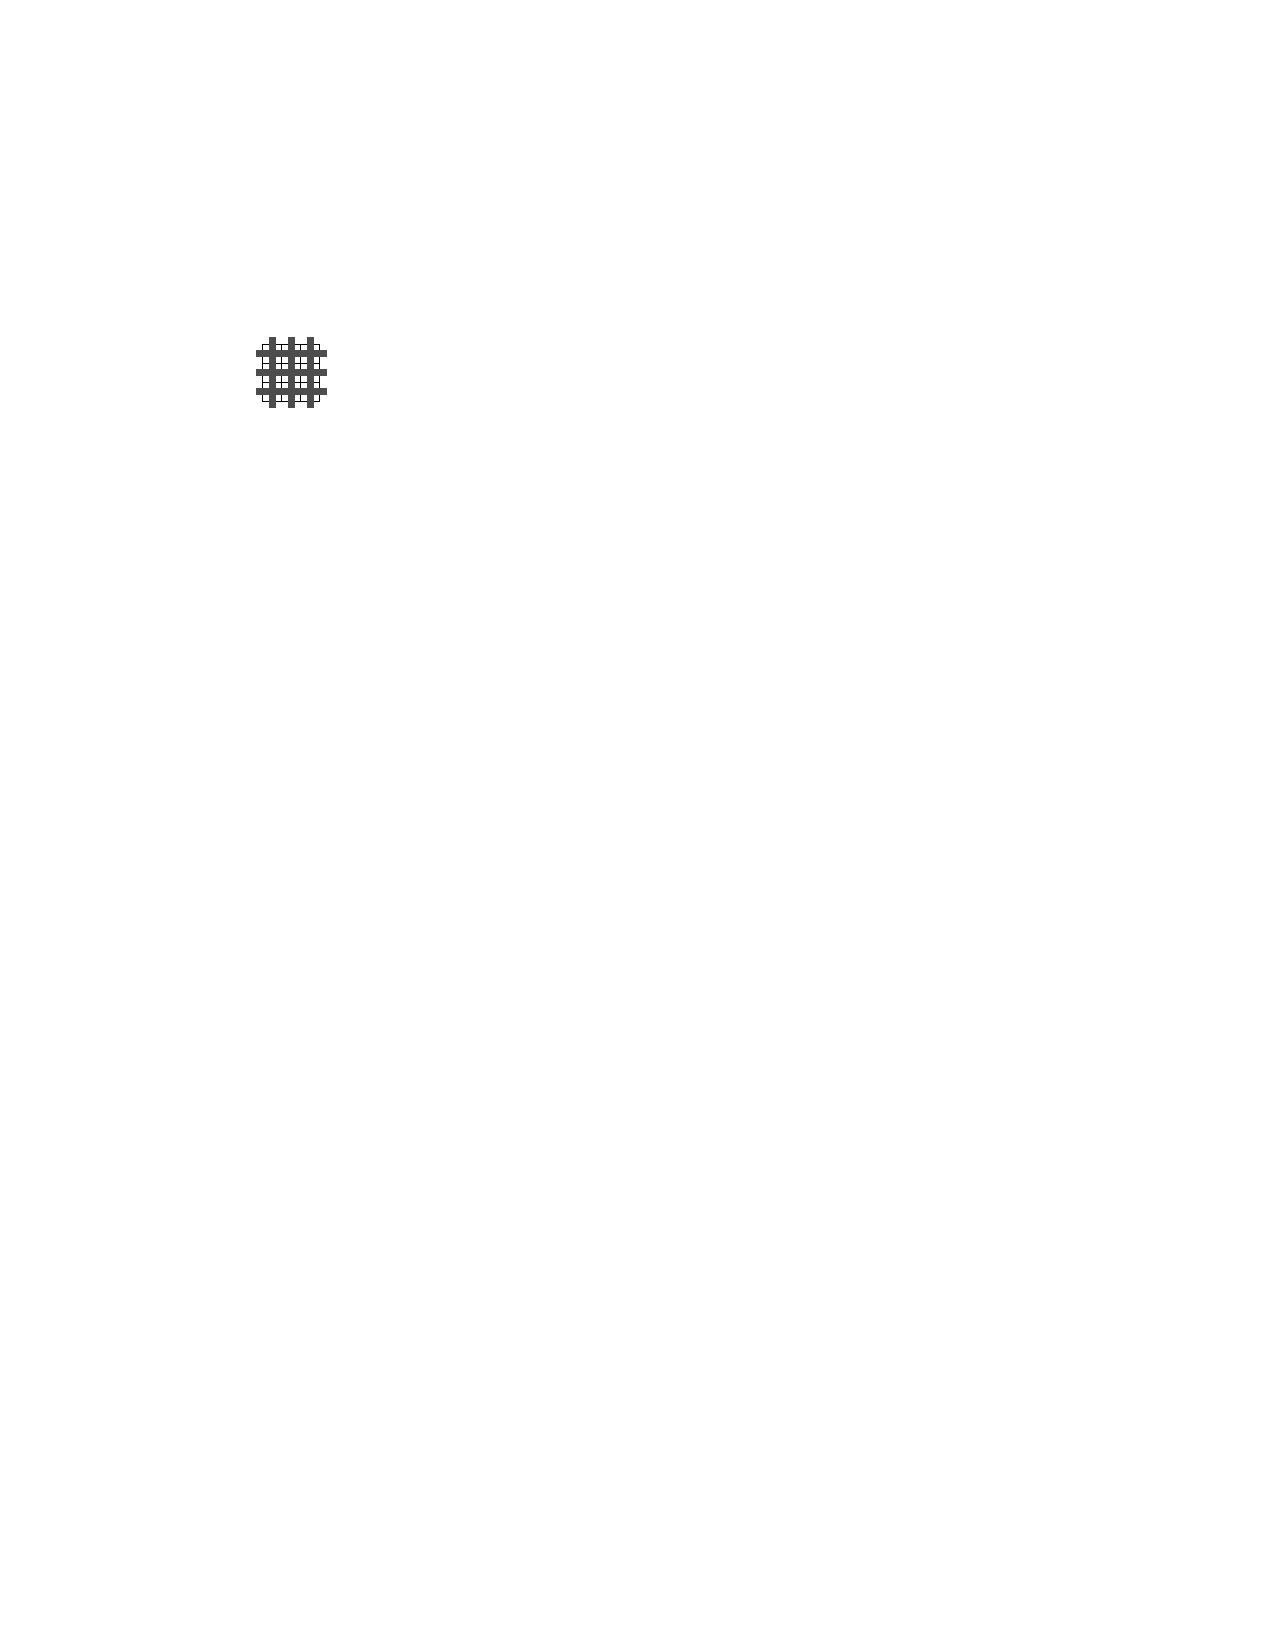
\includegraphics{misc/missing6}
\caption{\textit{Missing(6)} model}
\label{fig:missing6}
\end{figure}

An interesting observation is that the two most performant models also have the same number of backtracks. One of them is the model with nothing but channeling constraints, the other uses the \href{http://eclipseclp.org/doc/bips/lib/ic_global/occurrences-3.html}{\texttt{occurrences/3}} constraint which enforces arc-consistency. The first will detect when for a given \textit{row-column}, \textit{row-value}, \textit{column-value} or \textit{block-value} combination only one possible \textit{value}, \textit{column}, \textit{row} or \textit{position} remains. It will remove this value, column, ... from the domains of the other primal or dual variables\footnote{The difference between unequality constraints and channeling is explained in more detail in \cite{article:channeling}. Adding unequalities to the implementation slows down the search procedure because the channeling constraints already do this propagation and more.}. The second does the same ; it can propagate unequalities when the domain of a variable is reduced to a singleton but also knows when a value can be put in only one particular cell of a row, column or block. It is probably slower because the constraint itself is more generic than reification constraints.\\\par

A model combining the classic viewpoint with the fourth dual model was set up. Number of backtracks and runtimes are displayed in table \ref{tab:res2}.

\begin{snippet}[H]
\caption{Channeling constraints for the combined viewpoint model}\label{channeling}
\small
(multifor([Row,Column,Value], 1, N), param(Primal, Dual, K) do \\
    \qquad\#=(Primal[Row,Column], Value, Bool), \% reification \\
    \qquad block(K, Row, Column, Block), \% calls utility function to convert $R\times C\rightarrow B$ \\
    \qquad position(K, Row, Column, Position), \% calls utility function to convert $R\times C\rightarrow P$ \\
    \qquad\#=(Dual[Block,Value], Position, Bool) \% reification\\
)
\end{snippet}

The \texttt{first\_fail} heuristic generally outperforms \texttt{input\_order}. It considers variables with the smallest domain first, rather than considering variables in the order they were given. This increases pruning power as removing a value from the domain will remove a bigger part of the search tree because the branching count increases as you go down the tree (which is not necessarily the case when using \texttt{input\_order}). This tends to cause the number of backtracks to decrease. Unless the solution lies at the left side of the search tree generated by the \texttt{input\_order} heuristic performance will increase in comparison. \\\par

As for the \texttt{all\_different} constraints, more constraint propagation can be done when making use of \texttt{ic\_global} since it enforces bounds consistency rather than enforcing arc-consistency on the corresponding inequalities. This decreases the number of backtracks, sometimes at the cost of performance.

\subsection{CHR}

Some of the viewpoints considered previously were implemented in \texttt{CHR}, too. The runtimes are shown in table \ref{tab:res4}. The \texttt{first\_fail} variable heuristic and the \texttt{indomain\_min} value heuristic. These are easy to implement and generally perform quite nicely. The combined model generally performed at least as well as the worst of the two other models except when runtime was already low. This is to be expected ; the running times\\\par 

Because the channeling-only viewpoint performed best in ECLiPSe an attempt was made at implementing it in \texttt{CHR}. \\\par 

Due to a failed experiment\footnote{At some point a constraint \texttt{pos/4} was used to convert from \textit{row-column} combinations to the corresponding blocks and positions (e.g. \texttt{pos(2,3,1,6)}. This slowed down the algorithm a lot.} the focus was laid on adding redundant constraint instead of changing the viewpoint.

\begin{table}[h]
\footnotesize
\bgroup
\def\arraystretch{1.3}
\begin{tabular}{ccccccccc}
\multicolumn{1}{l}{} & classic & dual1 & dual2 & dual3 & boolean & laburthe & member & channeling \\ \hline
Total/Average & 1981/142 & 2694/193 & 3467/248 & 2178/156 & 1998/143 & 14270/1020 & 1267/91 & 688/50 \\
Total/Average (minimum) & 2628/27 & 3183/32 & 3148/32 & 2612/27 & 2715/27 & 59340/594 & 1909/20 & 2026/20
\end{tabular}
\egroup
\caption{Runtimes for the various viewpoints (ECLiPSe) - shown in milliseconds. The \texttt{first\_fail + indomain\_min} heuristics were used.}
\label{tab:res1}
\end{table}


%\setlength\arrayrulewidth{0.5pt}
%\taburulecolor{gray}
\begin{table}[H]
\footnotesize
\bgroup
\def\arraystretch{1.3}
\begin{tabular}{ccc|cc}
\multicolumn{1}{l}{}    & \texttt{input\_order} & \texttt{first\_fail} & \texttt{input\_order} (global) & \texttt{first\_fail} (global) \\ \hline
& classic - dual & classic - dual & classic - dual & classic - dual \\
\textit{lambda} & 495/4712 - 162/1715 &  149/977 - 72/523 &  22/3 - 17/0 & 22/3 - 19/0 \\
\textit{hard17} & 132/873 - 87/389 & 92/419  - 68/198 &  20/1 - 27/1 & 27/1 - 29/1 \\
\textit{eastermonster}  & 62/119 - 75/125 & 58/101 - 84/155 &  237/51 - 236/49 & 169/33 - 256/66  \\
\textit{tarek\_052}  & 72/193 - 68/200 & 62/130 - 59/137 &  370/61 - 324/63 & 224/35 - 180/34  \\
\textit{goldennugget} & 103/520 - 98/441 & 87/358 - 90/281 &  687/104 - 517/72 & 334/76 - 264/44  \\
\textit{coloin} & 368/2209 - 246/2288 & 61/83 - 55/80 &  249/88 - 675/194 & 79/8 - 63/10  \\
\textit{extra2} & 305/4652 - 172/2894 & 641/7690 - 392/4232 &  18/0 - 18/0 & 19/0 - 21/0  \\
\textit{extra3} & 530/4712 - 176/1715 & 166/977 - 93/523 &  22/3 - 17/0 & 22/3 - 19/0   \\
\textit{extra4} & 1445/15116 - 409/6087 & 234/2097 - 139/1031 &  23/4 - 19/0 & 22/3 - 19/0  \\
\textit{inkara2012} & 21/50 - 49/72 & 91/273 - 75/199 &  42/3 - 97/3 & 97/17 - 106/15  \\
\textit{clue18} & 220/1838 - 161/1977 & 93/439 - 96/493 &  272/69 - 207/47 & 12/8 - 62/6  \\
\textit{clue17} & 523/5520 - 329/3509 & 78/270 - 72/201 &  17/0 - 18/0 & 22/0 - 18/0  \\
\textit{sudowiki\_nb28} & 324/2851 - 501/4555 & 322/2221 - 455/3015 & 1083/413 - 1292/421 & 638/297 - 875/353  \\
\textit{sudowiki\_nb49} & 186/1078 - 127/749 & 88/655 - 137/672 & 246/48 - 201/40 & 224/58 - 275/62  \\\hline
Total/Average (ms) & 4782/342 - 2654/190 & 2216/159 - 1880/135 & 3302/236 - 3660/262 & 2013/144 - 2201/157   \\
Total/Average (backtracks) & 44443/3175 - 26716/1909 & 16690/1192 - 11740/838 & 848/61 - 890/64 & 542/39 - 591/42                          
\end{tabular}
\egroup
\caption{Results for the classic and alternative (dual) viewpoint (ECLiPSe) - shown as milliseconds/backtracks.}
\label{tab:res2}
\end{table}

\begin{table}[H]
\centering
\footnotesize
\bgroup
\def\arraystretch{1.3}
\begin{tabular}{ccc|cc}
\multicolumn{1}{l}{}    & \texttt{input\_order} & \texttt{first\_fail} & \texttt{input\_order} (global) & \texttt{first\_fail} (global) \\ \hline
\textit{lambda} & 0 &             &                           &                          \\
\textit{hard17}          &              &             &                           &                          \\
\textit{eastermonster}   &              &             &                           &                          \\
\textit{tarek\_052}      &              &             &                           &                          \\
\textit{goldennugget}    &              &             &                           &                          \\
\textit{coloin}          &              &             &                           &                          \\
\textit{extra2}          &              &             &                           &                          \\
\textit{extra3}          &              &             &                           &                          \\
\textit{extra4}          &              &             &                           &                          \\
\textit{inkara2012}      &              &             &                           &                          \\
\textit{clue18}          &              &             &                           &                          \\
\textit{clue17}          &              &             &                           &                          \\
\textit{sudowiki\_nb28}  &              &             &                           &                          \\
\textit{sudowiki\_nb49}  &              &             &                           &                          \\\hline
Total/Average           &              &             &                           &                          \\
Total/Average (minimum) &              &             &                           &                         
\end{tabular}
\egroup
\caption{Results for the combined (classic + dual) viewpoint (ECLiPSe) - shown as backtracks/milliseconds.}
\label{tab:res3}
\end{table}

\begin{table}[H]
\footnotesize
\centering
\bgroup
\def\arraystretch{1.3}
\begin{tabular}{cccc|cc}
\multicolumn{1}{l}{} & classic & dual & combined & channeling-only & dual (bis) \\ \hline
\textit{lambda} & 0 & 0 & 0 & 0 & 0  \\
\textit{hard17} & 0 & 0 & 0 & 0 & 0  \\
\textit{eastermonster} & 0 & 0 & 0 & 0 & 0  \\
\textit{tarek\_052} & 0 & 0 & 0 & 0 & 0  \\
\textit{goldennugget} & 0 & 0 & 0 & 0 & 0  \\
\textit{coloin} & 0 & 0 & 0 & 0 & 0  \\
\textit{extra2} & 0 & 0 & 0 & 0 & 0  \\
\textit{extra3} & 0 & 0 & 0 & 0 & 0  \\
\textit{extra4} & 0 & 0 & 0 & 0 & 0  \\
\textit{inkara2012} & 0 & 0 & 0 & 0 & 0  \\
\textit{clue18} & 0 & 0 & 0 & 0 & 0  \\
\textit{clue17} & 0 & 0 & 0 & 0 & 0  \\
\textit{sudowiki\_nb28} & 0 & 0 & 0 & 0 & 0  \\
\textit{sudowiki\_nb49} & 0 & 0 & 0 & 0 & 0  \\\hline
Total/Average & 0 & 0 & 0 & 0 & 0  \\
Total/Average (minimum) & 0 & 0 & 0 & 0 & 0                      
\end{tabular}
\egroup
\caption{Results for the CHR Sudoku solver - shown as backtracks/milliseconds. Dual corresponds to \texttt{dual4} in the ECLiPSe version, dual (bis) with \texttt{dual3}.}
\label{tab:res4}
\end{table}

%
% Hashiwokakero
% 

\section{Hashiwokakero}

Hashiwokakero is another Japanese logic puzzle published by the same company, in which islands have to be connected by bridges. Six constraints are to be respected, the last one being the connectedness constraint, i.e. that all islands have to be connected. What follows is a discussion of an implementation of two solvers of Hashiwokakero puzzles. One written in ECLiPSe, the other in \texttt{CHR}.

\subsection{ECLiPSe implementation}

A partial solution by Joachim Schimpf was provided. It did not enforce the connectedness constraint. Joachim defines four variables for each of the input puzzle's cells. They represent the number of bridges for each of the cell's directions (north, east, south, west). Then he enforces the five first constraints :
\begin{enumerate}
\item[1-2.] Bridges run in one straight line, horizontally or vertically. This is enforced with equality constraints, making sure that the number of bridges for a given direction of a given cell equals the number of bridges in the opposite direction of a neighbouring cell. A total of four equality constraints for every cell except those on the border, which may only have two or three neighbours\footnote{It can be noted that Joachim's code enforces both $A$\#=$B$ and $B$\#=$A$ in several cases. It has no effect on the runtimes.}.
\item[3.] Bridges cannot cross other bridges or islands. This is enforced by making sure that any cell that does not represent an island either has no horizontal or no vertical bridges.
\item[4.] At most two bridges connect a pair of islands. Joachim imposes this constraint by declaring the domains of the variables to be $[0\dots 2]$.
\item[5.] The number of bridges connected to an island must match the number $X$ on that island. A simple sum constraint ($N+E+S+W$\ \#=\ $X$) suffices to enforce this one.
\end{enumerate}

The connectedness constraint was enforced through the use of an analogous set of four variables ($FN,FE,FS,FW$) per cell, denoting the \textit{flow} for each of the cell's directions. Say the island at the upper left is said to be the sink, then if a flow can be assigned to all islands such that the sink's incoming flow equals the total number of islands minus one, the islands are sure to be connected. The net flow for each non-sink island needs to be one, for each cell it should be zero, and empty cells should have no flow. Most of these constraints can be implemented with equality constraints (the \texttt{ic} library enforces bound consistency for these), some of the others were implemented with the use of the \href{http://eclipseclp.org/doc/bips/lib/ic/EG-2.html}{$\Rightarrow$} (`implication') constraint.\\\par

\begin{snippet}[H]
\caption{Constraint stating that the flow in a bridge should be zero.}\label{hashi}
\small
N + E + S + W \#\textbackslash= 0 => FN \#= -(FS) \texttt{and} FE \#= -(FW) \texttt{and} FN + FE +FS + FW \#= 0
\end{snippet}

All of these constraints are active, meaning that when variables are, in a sense, `woken up', the domain of associated variables is updated accordingly.\\\par

The provided benchmarks are solved rather quickly by the solver. It generally takes a few milliseconds, even for the biggest board. If one makes use of the \texttt{most\_constrained} or the \texttt{occurrence} variable heuristic, runtimes increase. The \texttt{largest} or \texttt{smallest} heuristics perform even worse. This is due to the fact that these heuristics are more likely to label variables. Flow variables have larger domains and most of the values in their domain cannot partake in a solution. As a result, backtracks increase and runtimes do too.

\subsection{CHR implementation}

A \texttt{CHR} solver was also created. Because of the results of the previous experiments no special heuristic (such as \texttt{occurrence} or \texttt{most\_constrained}) was made use of. The solver generates \texttt{island/7} and \texttt{cell/4} constraints which associates islands and cells with their variables (representing the number of bridges in a given direction) and their number (in the case of islands). Every island has a corresponding \texttt{sum/3} constraint which gets updated every time any of the variables in its list is assigned. This corresponds to forward checking. The variables represent the number of bridges for a given direction and a given cell (or island). Instead of defining all these variables separately and enforcing $V_1=V_2$ equality constraints whenever they're supposed to be equal, shared variables are defined instead. This is done in the pre-processing step when the board is read. Because of this decision all but the second and the fifth constraint have to be enforced. The sum constraint was just described. The way the second constraint is dealt with is shown in code snippet \ref{hashi2}. As can be seen, the \texttt{in/2} constraint (and operator) is used to update domains.

\begin{snippet}[H]
\caption{Enforcing that no bridges can cross in \texttt{CHR}.}\label{hashi2}
\small
assign(Val,X), cell(\_,\_,X,Y)\ \#\ passive $\Longrightarrow$ Val > 0\ |\ Y\ in\ [0].\\
assign(Val,X), cell(\_,\_,Y,X)\ \#\ passive $\Longrightarrow$ Val > 0\ |\ Y\ in\ [0].
\end{snippet}

Two additional constraints were added to speed up the solver. The first is a generalised version of the \textit{`4 in the corner, 6 on the side and 8 in the middle'} technique. If an island's number equals twice its number of neighbours then it should be connected with each of these neighbours by a pair of bridges. This covers some of the special cases as \textit{`neighbour'} is defined more broadly as  \textit{`any island to which the island can still be connected with at a certain point'}\footnote{Let's give a concrete example. Say, an island has the number four and three neighbors. Nothing could be concluded before doing any searching. If at any point during search it becomes clear that one of the three neighbors can't be connected to the island, then two pairs of bridges need to be added to form connections with the remaining neighbours.}. As expected, it sped up the solver for all puzzles, almost cutting the total runtime by half.\\\par

The second constraint prevents isolation of some islands by stating that any two neighbouring islands, both with the number one or two, cannot be connected by that same number of bridges\footnote{Note that in the case of trivial boards with nothing else than two such islands enforcing this constraint would prevent the solution from being found.}. Only in the sixth puzzle did this speed up the search by about half a second due to the reduction in number of backtracks. Interestingly the constraint slows down puzzle two, as enforcing it changes the variable ordering leading to a stark increase in number of backtracks\footnote{Experiments with value heuristics (\texttt{indomain\_min}, \texttt{indomain\_max}) showed that changing the heuristic can have a large impact on the number of backtracks. The same holds true for variable heuristics. Part of the reason why ECLiPSe is a whole lot faster is that it enforces bound consistency for the sum constraints. In the sum constraints of the basic \texttt{CHR} solver only forward checking is done.}.\\\par

Some redundant constraints were already part of the basic solver. For example, if an island only has one neighbour, its sum constraint only contains one variable which can readily be assigned.\\\par

As for the connectedness constraints, both passive - and active versions were implemented. Because any initial solution generated without enforcing connectedness still tends to be connected anyways\footnote{At least in the case of the provided benchmarks. In the case of puzzle six and a two smaller boards that were added, the first solution isn't connected.}, any constraint propagation relating to flow tends to slow down the search procedure. Because of this the passive versions of the connectedness constraints outperform the active versions (having a total runtime of about 6 seconds for all six puzzles).\\\par

The passive checks can intuitively be understood as follows ; all paths from the sink to all corners of the board are tracked until all connected islands have been visited. If at that point any islands remain that haven't been visited, then the board is not connected.\par
As far as the implementation goes, a \texttt{connects/5} constraint is added for any two islands that \textit{can} be but aren't necessarily connected. This is done in the pre-processing step, where all the variables are defined. When at any point during the search procedure the number of bridges between islands is determined, then the corresponding constraint is replaced by a \texttt{connected/4} constraint which says that the islands \textit{are} connected. At the end of the search procedure the \texttt{connected/4} constraints are used to traverse all paths starting from the sink, and if any such connection remains that couldn't be reached from the sink, failure is reported.\\\par

In the case of puzzle six no solution could be found in a reasonable amount of time when the initial versions of the active connectedness constraints were used. The domains of the flow variables are quite large because the number of islands equals 140. While for most of these islands the flow can easily and uniquely be determined, 35 flow sum constraints are less trivial. Generally speaking, when a bunch of islands are connected in a circle (meaning that there is no \textit{`tail'}, i.e. every island is connected to at least 2 other islands) the solution isn't unique. It's what happens in puzzle six, where after cutting all the \textit{`tails'} a few circles remain (see figure \ref{fig:circles}).

\vspace{0.1cm}
\begin{figure}[H]
\centering
\begin{BVerbatim}[fontsize=\footnotesize]
              5 = = 4 = = 4 - - 3 = = 3
              |           |           |
              3 = 3 - 3 = 5           |
                                      3
                                      X
                                      X
          5 - - 2                     3
          X     |                     |
          5 = = 6 - - 6               |
                      X               2
                      X               |
                      6               |
                      X               3
            3 - 4     X               X
            X   X     X               X
            6 = 6 = = 7               4
                      |               X
4 - 4                 |               4
X   |                 |               X
4 = 5                 4 = 3 - 5 = 6 = 4
\end{BVerbatim}
%4 = 5 - 2 - - 3 = 3 - 4 = 3 - 5 = 6 = 4
\caption{Puzzle 6's remnant structure after removing all \textit{`tails'} for which the value of the flow variables is trivial to determine.}
\label{fig:circles}
\end{figure}

If the sum constraints relating to flow enforce bound consistency (as is the case in ECLiPSe), wrong values can more quickly be filtered out. Realizing this, a limited form of bound consistency was implemented. A correct solution was generated much more quickly as a result as non-connectedness of a given solution could be detected earlier on. Eventually the search procedure still got stuck on puzzle six, looking for a valid way to label flow variables. After taking it up a notch (by improving the bound consistency logic) the solver managed to find a solution to that puzzle in 8 seconds. Enforcing bound consistency for the other sum constraints as well reduced total runtime to about 5 \sfrac{1}{2} seconds (all six puzzles).

%
% Scheduling Meetings
% 

\section{Scheduling Meetings}

The last challenge is the scheduling of some meetings, taking into account the preferences of the various persons involved. A constraint optimization problem where the cost is a function of the end time of the last meeting and the number of `\textit{violations}' (people of lower rank having their meeting after that of people of higher rank). This number of violations is of secondary importance.\\\par

Weekend constraints are generated first. If a person doesn't want to meet on weekends then his or her meeting is not allowed to overlap with the first weekend that follows :
$$((S + \textit{StartingDay})\ \texttt{mod}\ 7) + D <  5$$
In the above constraint $S$ and $D$ represent the start and duration of the person's meeting. Making direct use of \href{https://www.eclipseclp.org/doc/bips/kernel/arithmetic/mod-3.html}{\texttt{mod/3}} leads to an instantiation error, necessitating the use of an auxiliary variable representing the result of the modulo operation.

\begin{snippet}[H]
\caption{Weekend constraints}\label{weekend}
\small
X :: 0..6, \% Weekend constraints\\
\_Q * 7 + X \#= Start + StartingDay,\\
X + Duration \#< 6
\end{snippet}

Precedence constraints and constraints assuring that no meetings overlap are generated last. The corresponding code is fairly trivial\footnote{Note that all code for this third challenge can be found in \texttt{/src/scheduling/scheduling.pl}.}. The fact that the meeting with the minister should come last is equivalent to adding $N-1$ precedence constraints with $N$ the total number of persons.\\\par

The cost function is defined as $(V_{max}\times E)+V$ where $V_{max}$ is the maximum number of rank violations, $E$ is the end time of the meeting with the minister and $V$ is the actual number of rank violations for a given solution. This ensures that whenever two solutions have a different $E$, the solution with the smallest $E$ will have the lowest cost (whatever the number of violations $V$). Yet if two solutions have the same end time $E$, then it's the number of violations $V$ that will determine what solution is best.

\begin{snippet}[H]
\caption{Calculating the number of violations. The cost function is defined as $MaxViolations * (StartTime_{minister} + Duration_{minister}) + Violations$}\label{cost}
\small
violations(N, Ranks, StartTimes, Violations, MaxViolations) :-\\
    \qquad(for(I, 1, N-1),\\
     \qquad fromto([], InViolations, OutViolations, ViolationList),\\
     \qquad param(StartTimes, N, Ranks) do \\
        \qquad\qquad Rank is Ranks[I], \\
        \qquad\qquad (for(J, I+1, N-1), \\
         \qquad\qquad fromto([], In, Out, List), \\
         \qquad\qquad param(Rank, Ranks, StartTimes, I) do \\
            \qquad\qquad\qquad OtherRank is Ranks[J], \\
            \qquad\qquad\qquad (Rank < OtherRank -> Out = [(StartTimes[I] \#> StartTimes[J])|In] ; \\
            \qquad\qquad\qquad (Rank > OtherRank -> Out = [(StartTimes[I] \#< StartTimes[J])|In] ; \\
            \qquad\qquad\qquad Out = In)) \\
        \qquad\qquad ), \\
       \qquad\qquad append(InViolations, List, OutViolations) \\
    \qquad), \\
    \qquad length(ViolationList, MaxViolations), \\
    \qquad Violations \#= sum(ViolationList).
\end{snippet}

An additional constraint was used for the cost function, stating that it cannot be smaller than $V_{max}\times D_{tot}$ with $D_{tot}$ the sum of all meeting durations. This makes a difference\footnote{In our tests the total runtime was reduced by a factor of 4 (not when making use of the \texttt{ic\_edge\_finder} version).}.\\\par

Some implied constraints were added to increase performance. In case two persons have a different rank but the same meeting duration and weekend preferences, a corresponding order on their start times can safely be imposed. This mustn't override the precedence constraints.\\\par

Table \ref{tab:sche1} shows the runtime for each benchmark. Two versions are considered ; one ensures that no two meetings overlap by imposing a \texttt{(}$S_1$+$D_1$ $\leq$ $S_2$\ \texttt{or}\ $S_2$+$D_2$ $\leq$ $S_1$\texttt{)} constraint for every such pair, the other version uses a global version of these same constraints provided by the \href{http://eclipseclp.org/doc/bips/lib/ic_edge_finder/index.html}{\texttt{ic\_edge\_finder}} library. It's clear that the global version outperforms the other one. The time it takes to propagate the constraints is usually compensated for by the reduction in nodes having to be considered due to the pruning of the search tree.\\\par

Instead of making use of implied constraints one can also tinker with the various heuristics provided by the \href{http://eclipseclp.org/doc/bips/lib/ic/search-6.html}{\texttt{search/5}} procedure. Some of those lend themselves to some benchmarks but not to others.\par
The \texttt{indomain\_min} heuristic performed better than \texttt{indomain\_max} as it is an optimisation problem after all, meaning that selecting the minimum starting time selects solutions with a smaller cost first. A solution with a lower cost will prune the search tree more.

\begin{table}[H]
\footnotesize
\centering
\bgroup
\def\arraystretch{1.3}
\begin{tabular}{ccc}
\multicolumn{1}{l}{} & \texttt{input\_order} & \texttt{input\_order} + \texttt{ic\_edge\_finder} \\ \hline
\textit{bench1a}  & 207 & 326 \\
\textit{bench1b}  & 135 & 180                                 \\
\textit{bench1c}  & 314   & 269                                 \\
\textit{bench2a}  & 3636   & 2110                                 \\
\textit{bench2b}  & 19269   & 2043                                 \\
\textit{bench2c}  & 371   & 366                                 \\
\textit{bench3a}  & 143   & 138                                 \\
\textit{bench3b}  & 386   & 389                                 \\
\textit{bench3c}  & 286   & 309                                 \\
\textit{bench3d}  & 201   & 333                                 \\
\textit{bench3e}  & 405   & 371                                 \\
\textit{bench3f}   & 506   & 413                                 \\
\textit{bench3g}  & 568   & 479                                 \\\hline
Total/Average     & 26422/2033   & 7721/594                       
\end{tabular}
\egroup
\caption{Benchmark results for the Scheduling Meetings challenge, shown in milliseconds.}
\label{tab:sche1}
\end{table}

%
% Conclusion
%

\section{Conclusion}

Three challenges were addressed in this report. For each of these, a solver was implemented in at least one language. The solvers could be improved upon by experimenting further with redundant constraints or even some custom-made heuristics. Generally, however, satisfactory results were obtained. Some of the experiments underline the importance of active (instead of passive) constraints, the value of simplicity and the usefulness of introducing redundancy.

% 
% References
%
\bibliographystyle{plain}
\bibliography{References}
\addcontentsline{toc}{section}{References}

%
% Appendix
%

\newpage
\appendix
\section*{Appendix}
\label{sec:appendix}
\addcontentsline{toc}{section}{\nameref{sec:appendix}}

\subsection*{Reflection}\label{sec:reflection}
\addcontentsline{toc}{subsection}{\nameref{sec:reflection}}

When implementing the Sudoku solver in CHR we took a glimpse at Thom's implementation. It's given in his book as a solution to some exercise. Once we understood his approach we had the tendency to implement the viewpoints by making use of the same strategy ; constraints representing variables, constraints representing values, a simple implementation of the \texttt{first\_fail} heuristic and forward checking. This worked well, but it wasn't the most creative thing to do. Further experimentation with other models, heuristics, redundant constraints, ... was our way to (hopefully) compensate for this.\\\par

We also would have liked to have improved the bound (and arc) consistency logic in the \texttt{CHR} Hashiwokakero solver for all sum constraints. Making better use of the tracer would have saved us a lot of time which could have made this possible.\\\par

Some questions were asked online after all the code had been written. There were four of them, all about Sudoku. One on how to enforce equality of lists (we already had the solution but wanted to be sure there was no better alternative). One on looping through a list which is a subscript of an array (we found the appropriate solution ourselves). One on the inner workings of \href{http://eclipseclp.org/doc/bips/lib/ic_global/occurrences-3.html}{\texttt{occurrences/3}}. And a final one on memory usage. Aside from a quick experiment with \href{https://eclipseclp.org/doc/bips/kernel/termcomp/TE-2.html}{\texttt{$\sim$=/2}} no code was rewritten as a result. None of the questions mentioned Sudoku. All the viewpoints were either thought of by ourselves or come from the literature that was cited in this report.

%\subsection*{Workload}\label{sec:workload}
%\addcontentsline{toc}{subsection}{\nameref{sec:workload}}

\subsection*{Overview of the Code}\label{sec:code}
\addcontentsline{toc}{subsection}{\nameref{sec:code}}

\begin{table}[H]
\footnotesize
\centering
\bgroup
\def\arraystretch{1.3}
\begin{tabular}{llc}
Folder & File & Description \\ \hline
\texttt{/src/sudoku/} & \texttt{utils.pl} & \textit{Utility functions for Sudoku (CHR \& ECLiPSe)} \\    
\texttt{/src/sudoku/benchmarks/} & \texttt{benchmarks.pl} & \textit{Automatic benchmarking code} \\    
\texttt{/src/sudoku/benchmarks/puzzles/} & \texttt{*} & \textit{Sudoku benchmarks} \\    
\texttt{/src/sudoku/chr/} & \texttt{solver.pl} & \textit{Sudoku solver (CHR)} \\    
\texttt{/src/sudoku/chr/model/} & \texttt{*} & \textit{Sudoku viewpoints (CHR)} \\    
\texttt{/src/sudoku/eclipse/} & \texttt{solver.pl} & \textit{Sudoku solver (ECLiPSe)} \\    
\texttt{/src/sudoku/eclipse/model/} & \texttt{*} & \textit{Sudoku viewpoints (ECLiPSe)} \\\hline
\texttt{/src/hashiwokakero/eclipse/} & \texttt{solver.pl} & \textit{Hashiwokakero solver (ECLiPSe)} \\
\texttt{/src/hashiwokakero/chr/} & \texttt{solver.pl} & \textit{Hashiwokakero solver (CHR)} \\
\texttt{/src/hashiwokakero/benchmarks/} & \texttt{hashi\_benchmarks.pl} & \textit{Hashiwokakero benchmarks}  \\\hline
\texttt{/src/scheduling/} & \texttt{scheduling.pl} & \textit{Scheduling meetings solution} \\\hline  
\end{tabular}
\egroup
\caption{Overview of the source code. Any files in folders named \texttt{misc} have experimental code that isn't discussed in the report.}
\label{tab:code}
\end{table}

\subsection*{Submissions}\label{sec:submission}
\addcontentsline{toc}{subsection}{\nameref{sec:submission}}

The Tolinto registration as well as the submission of the report and code was done by Bruno Vandekerkhove.

\end{document}
